\documentclass[12pt]{article}
\bibliographystyle{unsrt}
\usepackage{a4}
\usepackage{graphicx}
\usepackage{url}
\newcommand{\ca}{\mbox{C$\alpha$}}

\title{Predicting the Quality of CDRH3 Antibody Loop Structural Models}
\author{Lilian M.\ Denzler and Andrew C.R.\ Martin\\
Structural and Molecular Biology, Division of Biosciences,\\
University College of London,\\
Gower Street,\\
London WC1E 6BT, UK
}

\begin{document}
\maketitle

\begin{abstract}
  Therapeutic antibodies have shown an unprecedented pace of
  development and have brought new hope for the treatment of numerous
  diseases. The bioinformatic tools for modelling antibody structures
  have become invaluable for antibody engineering and the development
  of therapeutic antibodies. The antigen-binding site consists of six
  hypervariable loops, also known as the Complementary Determining
  Regions (CDR), all of which can be modelled with adequate accuracy,
  except for one. It remains markedly difficult to model the third CDR
  loop of the antibody heavy chain. The CDR-H3 differs in length, has
  far greater sequence variability and has such a great structural
  diversity that modelling it is considerably harder.

  Many sophisticated approaches for antibody modelling, such as the
  abYmod software, have been developed. Although such efforts have
  improved prediction accuracy the results for the CDR-H3 loop are
  still inconsistent and require further improvement. Providing a
  confidence score for the structure predictions would aid in
  differentiating well-modelled structures from incorrectly modelled
  structures, giving the abYmod user a clearer understanding of the
  generated model reliability.

  We present a model quality predictor, combining domain knowledge
  with machine learning techniques to predict the accuracy of CDR-H3
  models generated by antibody modelling software such as abYmod. The
  newly developed predictor scored a Mathews Correlation Coefficient
  of 0.99, and can thus be described as highly reliable. The predictor
  is made available at \url{http://www.bioinf.org.uk/abs/qualiloop/}
\end{abstract}

\section{Introduction}

Antibodies are highly specialized proteins of the immune system that
are produced in response to a foreign substance, called an antigen. A
mature antibody binds a specific antigen with high affinity, while
only weakly interacting with other antigens, or not at all. This high
affinity, high specificity sets it apart from other pharmaceuticals.
Furthermore, in contrast with small drug molecules, antibodies can not
only bind pockets, but also flat, concave or even convex
surfaces\cite{Tavers2001}. Their unique characteristics have enabled 
researchers to develop efficient antibody drugs for treating cancers,
autoimmune disorders, infectious diseases and many more\cite{Lu2020}.
Their ability to target an immense variety of antigens allows for
endless possibilities in application. The global market size was
valued at USD 130.9 billion in 2020, estimated to grow 223.7 billion
by the end of 2025 at a compound annual growth rate of
11.31\%\cite{market2020}. Four of the top 10 best-selling drugs in
2020 were monoclonal antibodies\cite{Urquhart2021}.

In order to rationally design therapeutic antibodies, knowledge of
their structure is essential. The acquired structural information can
be used to increase binding affinity to a target of interest,
predicting both the exact binding site and the antibody stability as
well as assessing immunogenicity\cite{Abhinandan2007}. As
experimental structure determination is very costly and time
consuming, computational predictions of an antibody's structure are
used to streamline the process.

Antibodies consist of a heavy and a light chain, which are linked by
disulphide bonds. The N-terminal domain of each makes up the variable
fragment (Fv), which contains the complementarity determining regions
(CDRs). The antigen binding site is composed of six CDRs, also known
as hypervariable loops. All except one of these loops can be clustered
into a limited number of canonical structures. Therefore, modelling
these loops with adequate accuracy is commonly
achievable\cite{North2011,Weitzner2015}. However, the CDR loop 3 of
the 
heavy chain (CDR-H3) has a far greater sequence variability due to the
processes of V(D)J recombination and somatic hyper‐mutation and its
structure has remained unclassifiable\cite{Finn2016}. The variety in
structure is so great, that its structural diversity is remarkable
even compared to other protein loops\cite{Regep2017}. It was found
that over 75\% of CDR-H3 loops do not have a sub-{\AA}ngstr\"{o}m non-antibody
structural neighbour, as well as that 30\% of CDR-H3 loops have a
completely unique structure compared with under 3\% for all other
loops on average\cite{Regep2017}.

Apart from being the most structurally diverse, the CDR-H3 loop is
also the most important for antigen binding, being located at the
center of the binding site and forming the most contacts to the
antigen\cite{MacCallum1996}. In fact, it was demonstrated that
differences in this loop alone were sufficient to enable otherwise
identical antibodies to distinguish between various
antigens\cite{Xu2000}.

According to the Kabat definition, the CDR-H3 loop is made up of the
residues 95--105 (Kabat numbering scheme\cite{Kabat1992}) in the heavy
chain, with a potential insertion site at position 100. The
possibility of such an insertion of a varying number of residues leads
to a large range of loop lengths, with bovine antibodies being
exceptionally long (Figure~\ref{fig:loopdist}).

\begin{figure}
  \centering
  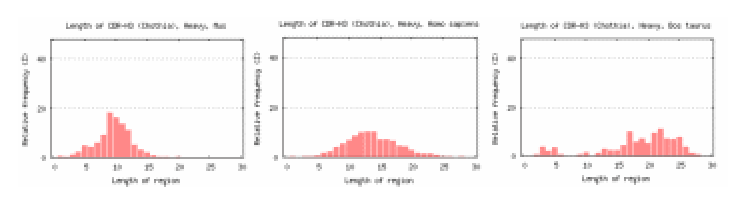
\includegraphics[width=\linewidth]{loopdist.eps}
  \caption { Distribution of CDR-H3 loop lengths in mouse (left),
    human (centre) and cow (right). Mouse and human antibody CDR-H3s
    have a unimodal, yet almost normal distribution with a range of
    $\sim$4--28 and 4--38 respectively. The length cut-off for CDR-H3s
    depicted above is 30 amino acids. Bovine antibodies with
    significantly longer CDR-H3 loops than depicted here exist,
    reaching a length of 67 amino acids and
    above\protect\cite{Wong2015}.}  
  \label{fig:loopdist}
\end{figure}

For shorter loops, a higher prediction accuracy can be achieved than
for longer CDR-H3 loops. This was also shown by the Antibody Modelling
Assessments (AMA), two blind contests that required researchers to
build structural models from antibody sequences. The CDR-H3 loop
modelling quality achieved at the contests was on average much lower
for loops of longer lengths\cite{Almagro2011,Almagro2014}.

Several different approaches for generating three-dimensional
structure models from antibody sequences exist such as
RosettaAntibody\cite{Sircar2009,Sivasubramanian2009}, 
ABodyBuilder\cite{Leem2016}, PIGSPro\cite{Lepore2017} and abYmod,
UCL's in-house software developed by Prof.\ Martin. One of the most
used methods is RosettaAntibody, which implements template selection
and ab initio CDR-H3 loop modelling using loop fragments and employing
specific angle restraints which bias the conformational space towards
so-called `kinked' loops\cite{Schoeder2021,Weitzner2017}. In
contrast, ABodyBuilder uses a database search algorithm
(FREAD\cite{Choi2010}) for CDR loop modelling.

In this project abYmod is used, which is to be found at
\url{http://abymod.abysis.org/}. The program utilizes extensive canonical
class definitions, VH/VL angle prediction and a large database of loop
structures (LoopDB) for CDR-H3 modelling to achieve optimal
results. Upon inputting an antibody sequence, abYmod assigns the
canonical class using a set of key residues\cite{Martin1996}and where
an exact match is not possible, a nearest match is made. Then, the
program identifies the 10 best overall-matching PDB files according to
sequence identity for the light and heavy chain. Of these, the best
template is then identified for each CDR using sequence similarity and
identity. In general, modelling the antibody using the single best
overall-matching template works best and the CDR-specific templates
are used if there is no canonical match. The VH/VL packing angle is
then determined either using machine learning or the chosen template
structure for one of the chains. CDR specific templates, if selected,
are grafted onto the framework. If there is no template of the correct
length for CDR-H3, the loop is built using the LoopDB database,
containing CDR-H3-like loops from all proteins. Finally, Gromacs energy
minimization software is used to optimize the model. This method has
proven very effective and preliminary analysis suggests the method
achieves comparable results or outperforms other modelling software
(see results section).

Using these mentioned modelling methods, framework regions can
generally be predicted with great accuracy (with better than 1\AA\
RMSD\cite{Almagro2014}), as one can often find a very similar
structure for the homology modelling process.  However, the CDR loops
are not as easily predicted due to their great diversity. If the
canonical conformation of CDR loops 1--5 can be identified, they too
can be modelled rather well, often within 1\AA\ RMSD, for CDR-H3 loops
the average is usually above 3\AA\cite{Almagro2011}.

ABodyBuilder is a modelling server that provides the user with a
confidence score for each region (e.g.\ CDR-H2) of the antibody
model. The given score is the probability that a specific region
(e.g.\ CDR-H2) will be will be modeled within a specific RMSD
threshold\cite{Leem2016}. Thus, it can be used to obtain an expected
RMSD value for a given probability (default 75\%). For the CDR-H3 this
score is calculated as a function of the loop length.  The confidence
scorer is described as robust, but less accurate in the case of CDR
loops due to the lack of data\cite{Leem2016}. ABLooper also provides a
confidence metric for the CDR-H3 loop model, which is estimated by the
diversity of a set of predicted conformations for the same
loop\cite{Abanades2022}. However, it remains unclear whether a high
prediction diversity score points towards loops with multiple
conformations or a low quality model. Furthermore, it remains unclear
how well the generated diversity score reflects model
quality\cite{Abanades2022}.


Modelling the CDR-H3 loop is a hurdle for in silico development of
therapeutic antibodies. Currently, there is no definite, reliable way
to determine how accurate a generated structural model is within the
H3 region. Therefore, the aim of this project will be to produce a
user-friendly predictor of CDR-H3 model quality. The predictor will give
the user an RMSD-range in {\AA}ngstr\"{o}ms, in which the generated model lies
with a high probability. Making such a confidence score available via
the web interface of the in-house modelling software abYmod is a
future goal. Such a score is not provided by most modelling programs
and would thus be a novel addition.  This information can guide the
user in the antibody engineering process. The user has the choice to
determine whether the model is to be used in the intended way, or
whether the model should be re-worked.

\section{Results}
To asses the predictive power regarding the CDR-H3 loop, the software
was tested on a test-set of antibody structures used in the 2014 and
2011 Antibody Modelling Assessments
\cite{Almagro2011,Almagro2014}. As the results depicted in
Figure~\ref{fig:AMA} show, abYmod achieves results similar to, or better than
other modelling programs. However, the outliers with very high RMSD
values increase abYmod's RMSD average. The predictor in this work
would aim to identify such outlier models.

The predictive power of any machine learning model is largely
dependent on the quality and size of the dataset it was trained on. As
this is a non-linear, complex, multi-class classification problem, a
substantial amount of data was required. Thus, an extensive, verified
dataset of antibody structures called abYbank/AbDb\cite{XXXX},
established by Prof.\ Andrew Martin, was utilised (1924 non-redundant
structures). The root-mean-square deviation (RMSD) value, a measure of
distance between backbone \ca\ atoms of superimposed crystal structures
and modelled structures, is calculated (see methods). This metric for
model quality was used to classify models.

\begin{figure}
  \centering
  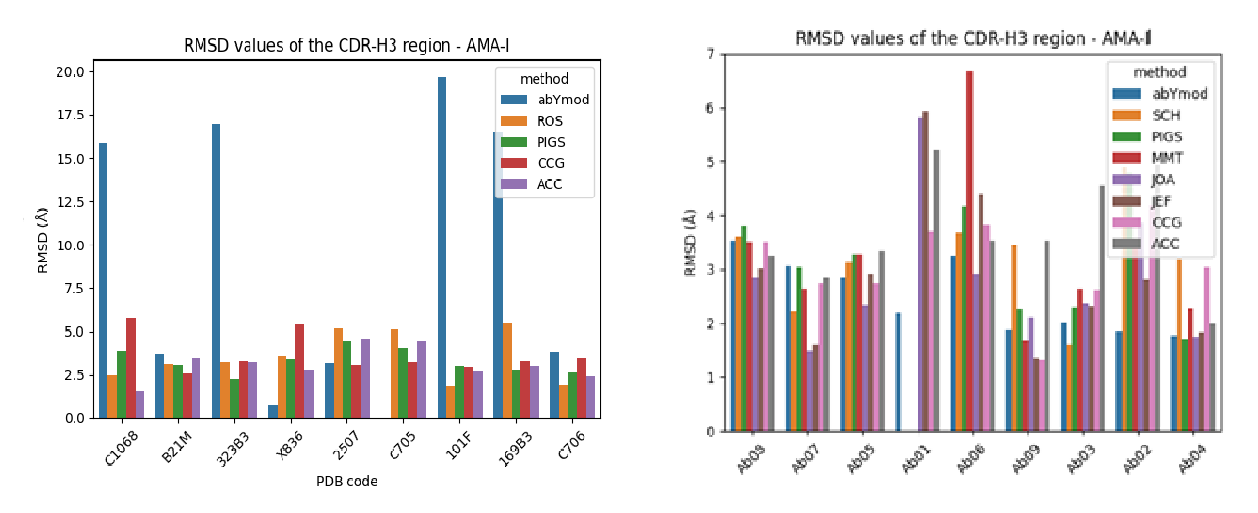
\includegraphics[width=\linewidth]{AMA.eps}
  \caption {RMSD values of the CDR-H3 loop for structures from the
    Antibody Modelling Assessment I (2011) and AMAII (2014). abYmod
    outperforms other modelling software in some instances, but also
    has much lower accuracy in few outlier cases. (left: an abYmod
    structure for C705 could be generated, yet the RMSD calculation
    failed. Right: Ab01 is the rabbit antibody PDB:4MA3, which was
    excluded in the CDR-H3 modelling stage in AMAII due to
    difficulties modelling the overall structure previously. Ab01 is
    shown for the methods, where generated models were adequate for
    RMSD calculation.)}
  \label{fig:AMA}
\end{figure}

The full pipeline for creating the final machine learning model that
will predict model quality by giving its RMSD range starts with a
feature-set calculation using the antibody sequence. The feature set
includes many different attributes linked to sequence, physical
characteristics, interactions, etc., within as well as outside of the
loop. There is a plethora of information to train our classifier on,
including packing quality, protrusion, hydrophobicity, pseudo-energy
(see protrusion, hydrophobicity, pseudo-energy (see methods for
details). The sequence logo (Figure~\ref{fig:logo}) visualizes amino acid
occurrence within the loop sequence, elements of which can be
extracted as features \cite{Thomsen2012,Shaner1993}.

\begin{figure}
  \centering
  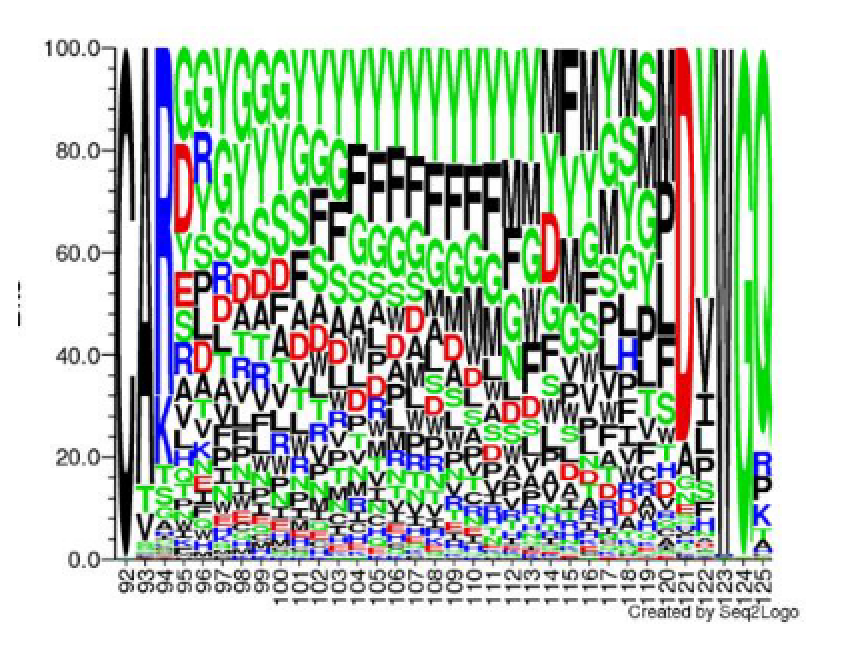
\includegraphics[width=\linewidth]{logo.eps}
  \caption {Sequence Logo of the CDR-H3 loop sequence. Data on amino
    acid occurrence taken from \protect\url{http://abymod.abysis.org/} Visualized
    using Seq2Logo.}
  \label{fig:logo}
\end{figure}

After creating the feature dataset, it is pre-processed (cleaning,
scaling, encoding, see methods for details). Structures with a
resolution below 4\AA\ were removed given their low quality. Identical
whole antibody structures were removed from the dataset, while
instances of different antibodies that matched in loop sequence were
not removed. Models of some of these structures with the same loop
sequence differ significantly. The few large RMSD ranges may stem from
low resolution, e.g.\ the highest datapoint contains a structure with a
resolution of 3.00~\AA.  Residue differences near the loop may also
explain the conformational difference. Some of these structures are
complexed while others are not, which may also affect the loop
structure.


The dataset was also screened for any models which abYmod created
using a template sequence from LoopDB, a database of CDR-H3 like loops
from all proteins. This was not the case for any of our structures.

The target data (i.e.\ RMSD values) are then transformed from numerical
values to nominal values so that they can be used for
classification. In order to define these nominal categories, the total
RMSD range must be divided into categories. This is done either by
creating uniform classes i.e.\ 1--2~\AA, 2--3~\AA\ (the optimal size of which
must be determined), etc.\ or by creating balanced classes. When
creating balanced classes, the upper and lower thresholds of a
category are chosen in such a way that each class contains an equal
number of instances. This approach is chosen to counteract the
skewness of the RMSD distribution. However, this was found to
negatively affect the final model's predictive power. Therefore,
uniform classes were used.

They are also transformed into a set of binary values according to a
list of RMSD thresholds. This is done so that binary models can be
trained, which will predict the probability e.g.\ that the model's RMSD
is above 2~\AA, 2.2~\AA, 2.4~\AA, and so on. The number of binary
classifiers incorporated into the first layer have a great effect on
the final model, the general trend being that the more binary
classifiers are used, the better the nominal prediction.

\subsection{Feature Encoding and Selection}

As some features are in the form of amino acid codes, these must be
encoded before they can be passed to a machine learning model. The
encoding strategy often determines how efficiently the model learns
and how much information can be extracted. Different strategies were
employed to represent followed by BLOSUM62 and NLF encoding. The
physiochemical encoding strategy was implemented for all models, being
the most effective. However, PCA-3 BLOSUM62, a dimensionality-reduced
BLOSUM62 encoding method achieved comparable results.

Feature selection was conducted to improve the ML model's learning
capacity. A high-dimensional feature dataset bears the risk of
introducing excessive noise, facilitating model overfitting and can be
responsible for an overall decrease in model performance and
stability. Each additionally inputted feature forces the model to
handle a more complex task, which consumes excess computational power
and time and leads to overfitting of the model.

Our model is trained on different feature sets selected using manual
selection as well as algorithmic selection strategies, in order to
determine the most effective feature selection method. None of the
feature selection methods was a best fit for all models.

After the data is processed, it can be fed into different machine
learning models. Different model types are investigated, as the most
suited model-type has to be heuristically determined. We decided on
the following list, which includes some of the most commonly used
algorithms: logistic regression, linear discriminant analysis,
K-nearest neighbours classifier, decision tree classifier, Gaussian
NB, random forest classifier, support vector machine,
probability-based voting (also known as soft voting) and extreme
gradient boosting (XGBoost)\cite{Chen2016}.

The best model, and its best hyperparameters, are then determined for
each binary RMSD target. The set of binary models outputs a number of
predictions that give the likelihood of the model having an RMSD above
the threshold value of the respective model. These predictions are
then added to the feature set, which a top-layer classifier is then
trained on. Thus, a quasi-voting-system is incorporated into the final
classifier, in which a set of weaker classifiers vote on the model
quality.

\subsection{Hyperparameter Optimization}
In the process of hyperparameter optimization, the configuration of
model parameters which results in best performance is selected. This
is usually a computationally expensive and manual procedure.

In an effort to automate this process, a population is defined for
each model type, so hyperparameter optimization can be conducted
automatically for each model and seamlessly integrated into the full
model creation process. Two different methods for hyperparameter
optimization were tested. The first is a hybrid approach of randomized
search and grid search, the second uses a genetic algorithm for
optimization. The genetic algorithm was found to achieve slightly
better results and was selected for all models.

\subsection{Model Performance}
The overall best final model is composed of several different binary
classifiers, with an extreme gradient boosting (XGBoost) top-layer
nominal classifier. Features were selected using random forest feature
selection. A final MCC value of 0.99 could be achieved for a model
using the abYmod log file as input as well as the loop model file
itself. This value slightly dropped to 0.92 if no such log file was
given. This is mainly due to the fact that the template sequence
abYmod used to generate the model is unknown in the latter case.

The classifier predicts whether a model has an RMSD of below 2~\AA,
between 2--4~\AA, or above 4~\AA. These cutoff values were selected
based on the observation that abYmod generally produces a model with
RMSD below 4~\AA. Incorrectly modelled structures (Figure~\ref{fig:AMA}) may
be identified by screening for structures estimated to have an RMSD
above 4~\AA. If a very high-quality model is needed one should also
exclude models above 2~\AA.


\section{Methods}

\subsection{Computing}
All machine learning and feature selection and hyperparameter
optimization algorithms were implemented in Python. The Scikit-learn
library was used for training models, the
Yellowbrick\cite{Bengfort2021} library was utilized for
visualization. All code is available at
\url{https://github.com/LilianDenzler/qualiloop}

The code was run under CentOS 7 on an 8-core virtual machine on an
Intel Xeon 4208 CPU with 16Gig RAM.

\subsection{Data Pre-Processing and Preparation}
Handling Null Values and Duplicates: The dataset containing target
RMSD values, and the calculated features was screened for null
values. If a feature column contained more than 5\% null values, it
was dropped (none removed). Rows that contained any null values were
removed from the dataset (11 rows in total).

\subsubsection{Duplicate Screening}
Using AbDb's redundancy information it was ensured that no antibodies
were present in the dataset more than once. The dataset is
additionally screened for duplicate instances.

\subsubsection{Scaling}
Normalization and Standardization are tested as scaling methods. Both
approaches are greatly influenced by outliers, and such datapoints are
ideally removed for optimal scaling. Here we define outliers as
datapoints that lie over 1.5 times the interquartile range (IQR) below
the first quartile or above the third quartile. The IQR is defined as
the range between quartile 1, i.e.\ the median of the lower half of the
data, and quartile 3, i.e.\ the median of the upper half of the
data. However, across all features there are a total of 632 outlier
values and removing such a large number of datapoints is not a viable
option. A robust scaler was also used, which uses statistics that are
robust to outliers. The median is set to zero and numerical features
are scaled to the interquartile range.

\subsubsection{BLOSUM 62 encoding}
The BLOSUM62 matrix reflects the frequencies of amino acid
substitutions within a locally aligned, conserved regions of proteins
with at least 62\% similarity. Each amino acid is represented by a row
(or column) of the BLOSUM62 matrix. Dimensionality reduction
techniques are employed: Principal Component Analysis (PCA),
Independent Component Analysis (ICA), projection-based methods (t-SNE,
Isomap). Three components were used as features.

\subsubsection{Physiochemical Feature Encoding}
In a paper by L.~Nanni and A.~Lumini a new encoding technique is
presented which was developed for machine learning classifiers. Many
physiochemical properties are calculated and transformed using a
non-linear Fisher transform for dimensionality reduction.  A vector of
length 19 is produced for each amino acid34.  In a paper on designing
a neural network for predicting the packing angle of the light and
heavy variable chain of an antibodies, A.C.R.~Martin and
K.R.~Abhinandan introduce an encoding method that produces a
four-dimensional physiochemical feature vector25. The amino acid
properties used are 1) the total number of sidechain atoms, 2) the
number of sidechain atoms in the shortest path from \ca\ to the most
distal atom, 3) the Eisenberg consensus
hydrophobicity\cite{Eisenberg1982}, 4) the charge.

\subsection{Dataset-splitting}
The final model was evaluated using a test set, separated from the
training set at the start in a 30/70 split (lock-box principle)
35. The performance of all individual sub-models of the first layer
are determined using stratified K-folds cross-validation (k=10) as the
dataset is imbalanced, being skewed towards lower RMSD values. The
method is differentiable from K-folds cross validation as it uses
stratified sampling instead of random sampling. This ensures each
class is represented, as the percentage of samples for each class are
preserved.

A validation set, usually used for testing during the optimization
stage will be omitted in favour of stratified K-folds cross-validation
(k=10)\cite{Krstajic2014,Kohavi1995}.

\subsection{Model Assessment} 
Model assessment must be considered at two levels as performance
metrics of binary and multi-class classifiers are calculated
differently and must thus be considered separately. The Mathews
Correlation Coefficient (MCC)\cite{Matthews1975} is deemed the most
informative, taking the ratios of the four confusion matrix categories
into account 39and is thus more reliable than the F1 score and
accuracy. It is also consistent for both binary and multi-class
problems and therefore well suited for our purpose.
 
\subsection{Feature Calculations}
\begin{figure}
  \centering
  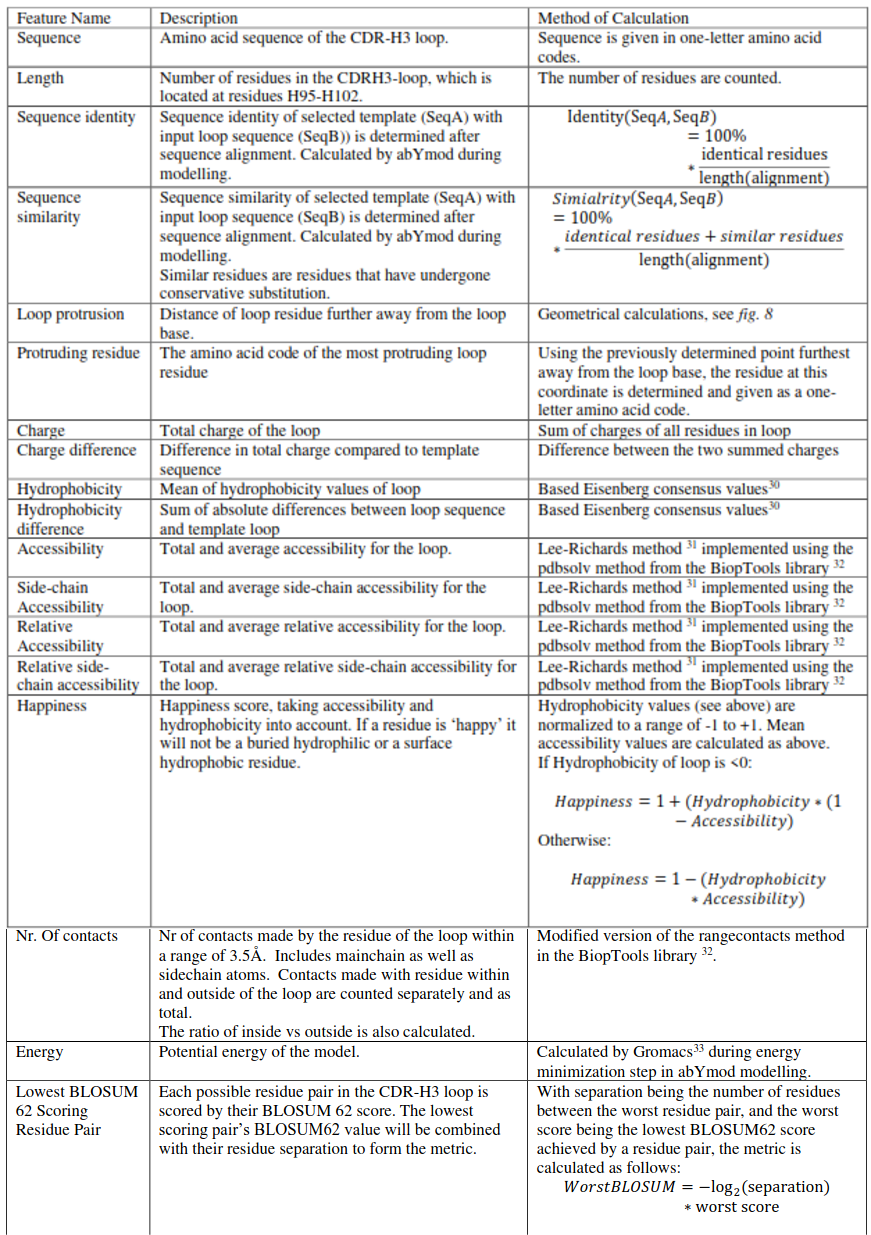
\includegraphics[width=\linewidth]{feature_table.eps}
  \caption {A summary of how different feature values were calculated.}
  \label{fig:feature_table}
\end{figure}

\begin{figure}
  \centering
  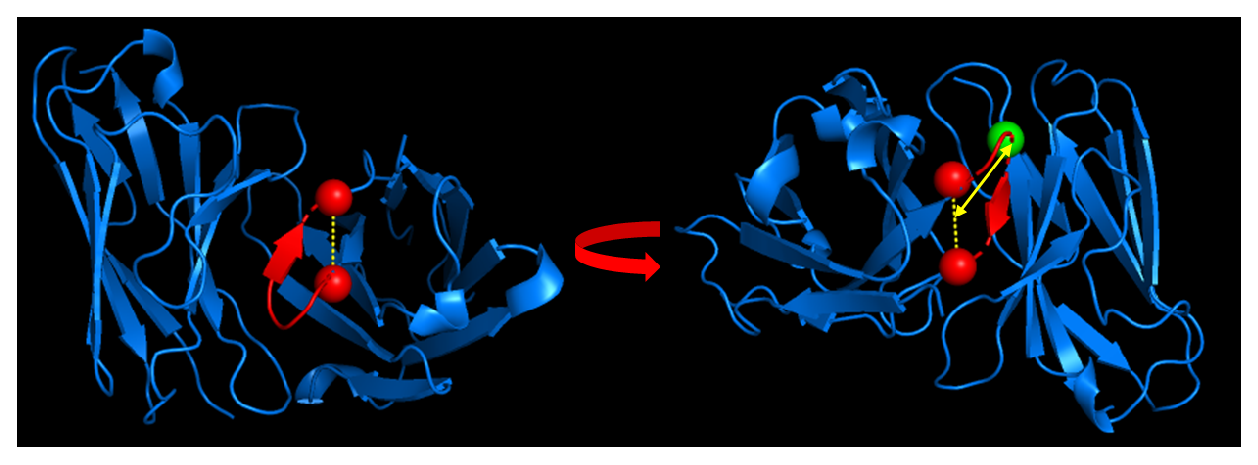
\includegraphics[width=\linewidth]{angle.eps}
  \caption {Diagram visualizing the process underlying the protrusion
    calculation. First, the base residues (i.e.\ H95 and H102, shown as
    red spheres) of the CDR-H3 (shown in red) are identified. Then, a
    line is drawn between the two \ca\ atoms of these residues (yellow
    dashed line). The distance of the \ca-atom of each residue in the
    CDR-H3 loop to this line is calculated. The residue which has the
    greatest distance to the line (shown as green sphere) is outputted
    as one-letter amino acid code and used as feature. The distance in
    \AA\ (depicted as yellow arrow) is used as the `protrusion'
    feature.}
  \label{fig:angle}
\end{figure}


\begin{figure}
  \centering
  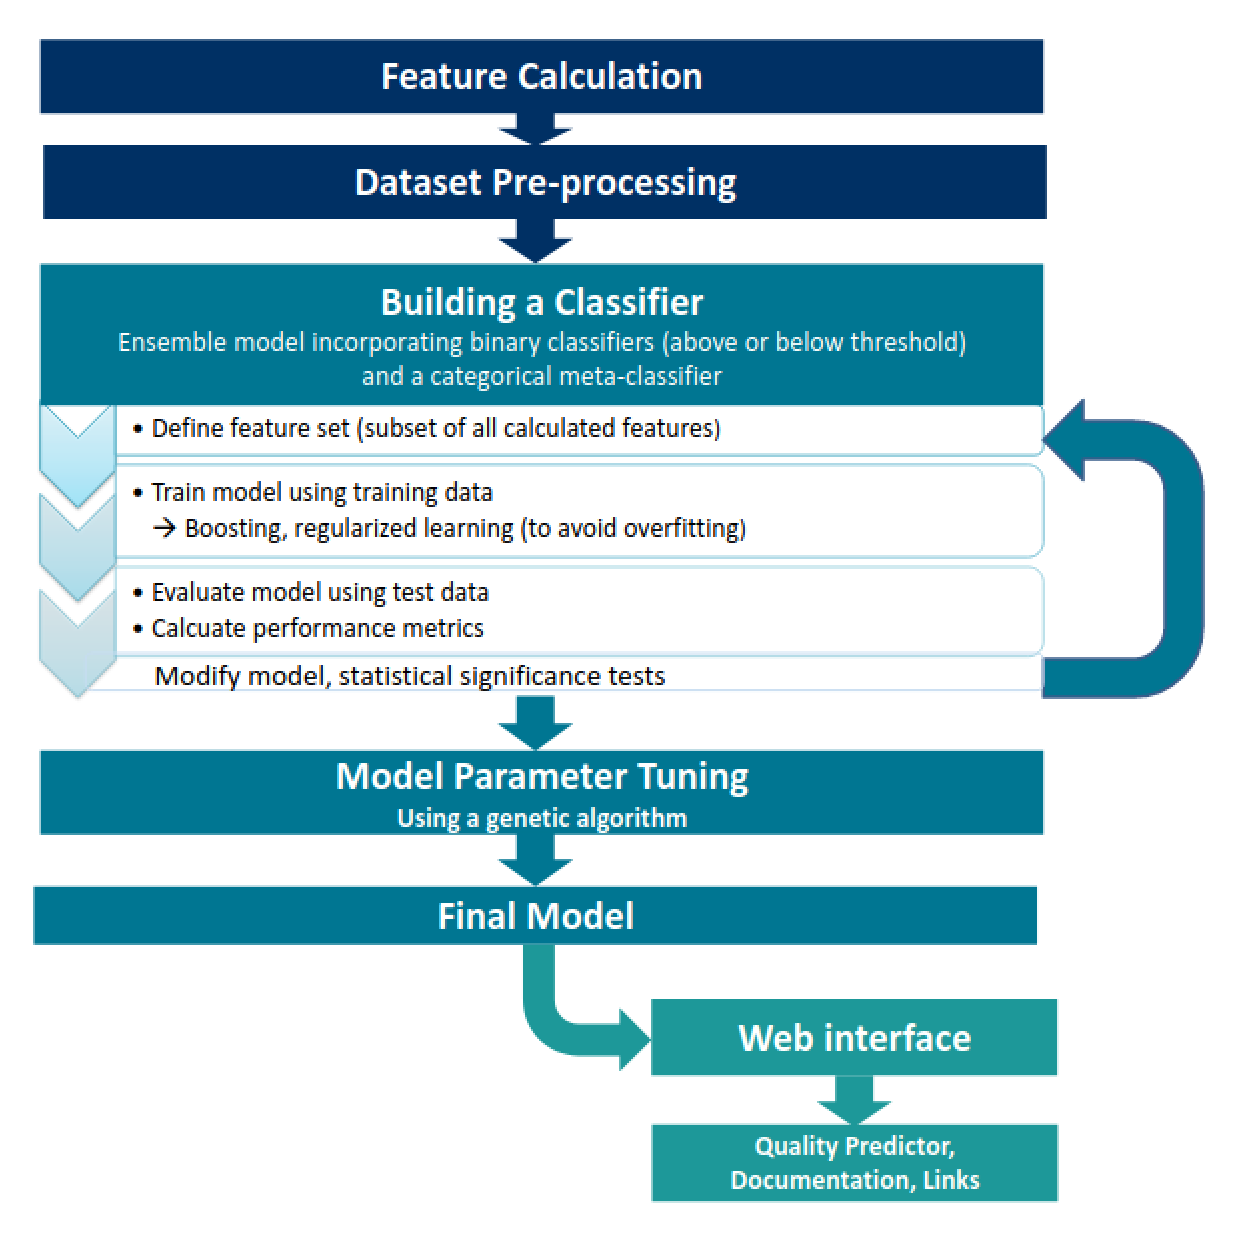
\includegraphics[width=\linewidth]{method.eps}
  \caption {Simplified pipeline for creating the final machine
    learning model that will predict model quality by giving its RMSD
    range.}
  \label{fig:method}
\end{figure}



\section{Discussion}
The results suggest that our presented classifier can differentiate
between well-modelled and less well-modelled CDR-H3 loop
structures. An MCC value of 0.99 was achieved, which underlines this
ability for accurate discrimination. Different methods for data
pre-processing, feature encoding, feature selection and hyperparameter
optimization were tested.

Feature encoding methods that were very high-dimensional
(one-hot-encoding, BLOSUM62, NLF) were found to be
unfavorable. Dimensionality reduction methods (Principal Component
Analysis (PCA), Independent Component Analysis (ICA), projection-based
methods e.g.\ t-SNE) were used on BLOSUM62 encoded matrices, which lead
to significant improvement. However, a physiochemical encoding
strategy was most effective.

The selection of features incorporated in the training set seemed to
be most important for effective learning. A multitude of methods were
tested. No one fit-for-all method for the different models could be
found. However, for our top-layer classifier in our final model
recursive feature elimination worked best.

A set of commonly used machine learning algorithms were tested, and
the best ML models were incorporated into the final ensemble model. A
stacked model approach (consisting of 23 binary classifiers and a
single top-layer nominal classifier) was shown to outperform single ML
models.

An MCC value of 0.99 was achieved for a classifier predicting whether
an input-model has an RMSD value below 2\AA, 2\AA--4\AA\ or above
4\AA.

Given that abYbank/AbDb is soon to be expanded by an additional
$\sim$2000 structures, classifier performance on models without a known
abYmod-template sequence may be improved by a larger dataset.

It is conceivable that the described predictor may also be
incorporated in the antibody modelling process as a low-quality filter
in the future, flagging certain structures for re-modelling.

In a future research project residue patterns in correlation with RMSD
may be analyzed. Possibly, one might identify certain sequence
patterns that make accurate modelling with abYmod more
difficult. Furthermore, separate classifiers according to loop length
can be built. Given that loop length is the most important determinant
of model quality, this approach may yield some insight into the
challenges of modelling shorter vs longer loops.

One could also conduct an analysis of the predictor's behaviour when
abYmod is forced to use LoopDB-based modelling. This might shed light
on whether the ML model presented in this paper is biased towards
abYmod's used source of template structures. It would also give an
indication of how well the predictor would work in combination with
other modelling software.

\bibliography{references}

\end{document}
